\documentclass[a4paper]{report}

\usepackage[in]{fullpage}

\usepackage[utf8]{inputenc}
\usepackage[T1]{fontenc}
\usepackage[french]{babel}

\usepackage{amsmath}
\usepackage{amssymb}
\usepackage{mathtools}
\usepackage[inline]{enumitem}
\usepackage[squaren,Gray]{SIunits}
\usepackage{sistyle}
\usepackage[autolanguage]{numprint}
\usepackage{xfrac}
\usepackage{bm}
\usepackage{color}
\usepackage[version=3]{mhchem}
\usepackage{multirow}
\usepackage{tabulary}

\newcommand{\diff}[1]{\mathrm{d}#1}

\let\oldvec\vec
\renewcommand{\vec}[1]{\oldvec{\bm{#1}}}
\newcommand{\uvec}[1]{\hat{\bm{#1}}}

\newcommand{\TODO}[1]{\colorbox{red}{\textbf{\textsc{TODO: #1}}}}

\newcommand{\e}[1]{\ensuremath{\cdot 10^{#1}}}

\makeatletter
\newcommand\reaction@[1]{\begin{equation}\ce{#1}\end{equation}}
\newcommand\reaction@nonumber[1]%
{\begin{equation*}\ce{#1}\end{equation*}}
\newcommand\reaction{\@ifstar{\reaction@nonumber}{\reaction@}}
\makeatother

\usepackage{fancyhdr}
\usepackage{layout}
\usepackage{geometry}
\usepackage{hyperref}
\usepackage{caption}
\newcommand{\reporttitle}{Synthèse de l’ammoniac}     % Titre
\newcommand{\reportauthor}{Simon \bsc{Boigelot} \\ Virgile \bsc{Goyens} \\ Corentin \bsc{Joachim} \\ Xavier \bsc{Lambein} \\Edward \bsc{Nicol}\\ Léa \bsc{Paulus}\\ Abbas \bsc{Sliti}} % Auteur
\newcommand{\reportsubject}{Projet Q3} % Sujet
\newcommand{\HRule}{\rule{\linewidth}{0.5mm}}
\newcommand{\copyrigh}{{\tiny \textregistered}}
\setlength{\parskip}{1ex} % Espace entre les paragraphes

\hypersetup{
    pdftitle={\reporttitle},%
     pdfauthor={\reportauthor},%
    pdfsubject={\reportsubject},%
    pdfkeywords={rapport} {vos} {mots} {clés}
}









\setlength{\headheight}{12pt}
\setlength{\headsep}{12pt}

\pagestyle{fancy}
\lhead{\leftmark{}}
\rhead{P3 - 2014 - gr54}
\cfoot{\thepage{}}


\begin{document}
\begin{titlepage}


\begin{center}

% Upper part of the page

\textsc{\Large Université Catholique de Louvain}\\[0.5cm]

\textsc{\LARGE Rapport de projet du troisième quadrimestre}\\[0.2cm]
\textsc{\LARGE LFSAB1503}\\[0.2cm]

% Title
\HRule \\[0.2cm]
{\huge \bfseries ERRATA :Synthèse de l'ammoniac}\\
\HRule \\[0.2cm]

% Author and supervisor
\begin{center}
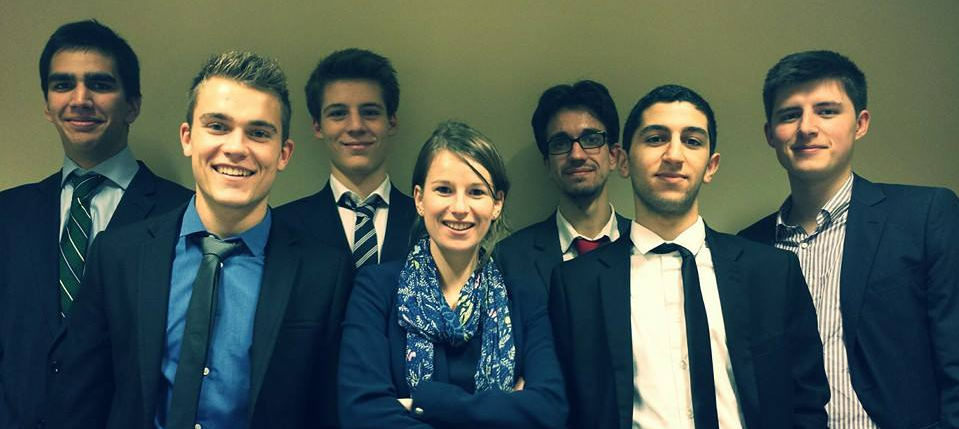
\includegraphics[trim=0cm 0cm 0cm 0cm, clip, width=15cm]{Shema/couverture2.png}
\end{center}
\HRule \\[0.2cm]
%inventer un petit texte cool :)
Dans le cadre de notre projet Q3, il nous a été demandé d'analyser et de proposer des pistes d'amélioration pour le procédé Haber-Bosch. En effet, la synthèse d'ammoniac rejette énormément de \ce{CO2}, c'est pourquoi nous avons exploré des solutions plus écologiques telles que le biométhane, l'hydrolyse ou encore des algues produisant de l'\ce{H2}.
\HRule \\[0.2cm]

\begin{minipage}{0.4\textwidth}
\begin{flushleft} \large
\emph{Auteurs:}
Groupe 1254\\ Simon \bsc{Boigelot} \\ Virgile \bsc{Goyens} \\ Corentin \bsc{Joachim} \\ Xavier \bsc{Lambein} \\Edward \bsc{Nicol}\\ Léa \bsc{Paulus}\\ Abbas \bsc{Sliti}
\end{flushleft}
\end{minipage}
\begin{minipage}{0.4\textwidth}
\begin{flushright} \large
\emph{Cours:} \\
FSAB1503\\
\emph{Groupe:} \\
1254\\
\emph{Tuteur:} \\
Vincent Destoop \textsc{}
\end{flushright}
\end{minipage}
\vspace{0.4cm}
% Bottom of the page

\begin{minipage}{0.3\textwidth}
\begin{flushleft}

\includegraphics[height=2cm]{Shema/logo_UCL_NEW_janv2013.JPG}
\end{flushleft}
\end{minipage}
\begin{minipage}{0.3\textwidth}
\begin{center}
{\large FSA12BA}\\
{\large \today}
\end{center}
\end{minipage}
\begin{minipage}{0.3\textwidth}
\begin{flushright}

\includegraphics[height=1cm]{Shema/epl-logo.jpg}
\end{flushright}
\end{minipage}
\end{center}
\end{titlepage}
\tableofcontents
%/!\ mettez la section et subsection dans laquelle l'eurreure se trouve !!!
\chapter{Bilan de masse}
\section{Bilan de masse du plant}
\subsection{bilan des réactions de synthèse}
\begin{center}
  \begin{tabular}{lccccc}
    &  \ce{CH4} & \ce{H2O} & \ce{CO} & \ce{H2} & \ce{CO2}  \\
    \hline
    $n_\text{init}$
    & $n_{i,\ce{CH4}}$ & $n_{i,\ce{H2O}}$ & \textcolor{red}{0} & 0 & 0  \\
    $n_\text{eq}$
    & $n_{i,\ce{CH4}}-R_1$ & $n_{i,\ce{H2O}}-R_1-R_2$ & $R_1-R_2$ & $3R_1+R_2$ & $R_2$
  \end{tabular}
\end{center}
\chapter{Analyse paramétrique}
\chapter{Mini-Hazop}
\chapter{Dimensionnement d'une soupape de sécurité}
\chapter{Activité de terrain}
\chapter{Annexes}
%\appendix
%\chapter{Bilan de masse: annexes}

\section{Système linéaire du bilan de masse}\label{appendix:matrix}

Pour éventuellement aider à comprendre le fonctionnement du bilan de masse, nous fournissons ici le système, sous forme matriciel, qui est à résoudre pour obtenir l'espace vectoriel $V$.

Dans l'ordre, les lignes de la matrice correspondent aux composés suivants : \ce{CH4}, \ce{H2O}, \ce{O2}, \ce{N2}, \ce{Ar}, \ce{CO},  \ce{CO2}, \ce{H2} et \ce{NH3}.
\[
\left(
\begin{array}{*{12}c}
  1 & 0 & 0 & 0 & 0 & 0 & 0 & -1 & 0 & -2 & 0 & 0 \\
  0 & 1 & 0 & -1 & 0 & 0 & 0 & -1 & -1 & 0 & -1 & 0 \\
  0 & 0 & 0 & 0 & 0 & 0 & 0 & 3 & 1 & 4 & 1 & -3 \\
  0 & 0 & 0 & 0 & 0 & 0 & 0 & 1 & -1 & 2 & -1 & 0 \\
  0 & 0 & 0 & 0 & -1 & 0 & 0 & 0 & 1 & 0 & 1 & 0 \\
  0 & 0 & .21 & 0 & 0 & 0 & 0 & 0 & 0 & -1 & 0 & 0 \\
  0 & 0 & .78 & 0 & 0 & 0 & 0 & 0 & 0 & 0 & 0 & -1 \\
  0 & 0 & .01 & 0 & 0 & -1 & 0 & 0 & 0 & 0 & 0 & 0 \\
  0 & 0 & 0 & 0 & 0 & 0 & -1 & 0 & 0 & 0 & 0 & 2
\end{array}
\right)
\left(
\begin{array}{*{1}c}
  n_{i,\ce{CH4}} \\ n_{i,\ce{H2O}} \\ n_{i,\text{air}} \\ n_{f,\ce{H2O}} \\ n_{f,\ce{CO2}} \\ n_{f,\ce{Ar}} \\ n_{f,\ce{NH3}} \\ R_1 \\ R_2 \\ R_3 \\ R_4 \\ R_5
\end{array}
\right)
= 0
\]


\section{Calcul des constantes d'équilibre}\label{appendix:const_eq}

Nous avons calculé les constantes d'équilibre des réactions 1 et 2 avec Matlab, à l'aide de l'expression suivante :
\[
    K = \mathrm{exp}\!\left( -\frac{\Delta G^0_m(T)}{RT} \right)
      = \mathrm{exp}\!\left( \frac{\Delta S^0_m(T)}{R} - \frac{\Delta H^0_m(T)}{RT} \right)
    \text.
\]
Dans cette expression, le symbole $\Delta$ correspond à la différence entre les produits et les réactifs. Par exemple, $\Delta S^0_m(T)$ est la somme de l'entropie molaire des produits moins l'entropie molaire des réactifs.

Il est donc nécessaire d'obtenir $\Delta S^0_m(T)$ et $\Delta H^0_m(T)$. Ceux-ci sont calculés à l'aide des formules :
\[
    \Delta S^0_m(T) = \Delta S^0_m(T_0) + \int_{T_0}^T\! \Delta C_{p,m} \frac{\diff{T}}{T}
    \qquad\text{et}\qquad
    \Delta H^0_m(T) = \Delta H^0_m(T_0) + \int_{T_0}^T\! \Delta C_{p,m} \diff{T}
    \text.
\]
Enfin, la différence de capacités calorifiques molaires $\Delta C_{p,m}$ qui apparait ici est obtenue, sous forme de polynomes de $T$, dans des tables thermodynamiques. Il en va de même pour l'enthalpie et l'entropie à la température de référence $T_0$.

Nous avons donc tous les outils nécessaires pour calculer la valeur de $K$ dans les deux réactions du réformeur primaire. Il suffit simplement d'implémenter les formules dans Matlab pour obtenir les constantes d'équilibres utilisées dans le calcul du bilan de masse.


\section{Usage du programme Matlab}

Le programme Matlab se trouve dans le sous-dossier \texttt{/manager/}. Il s'agit de la fonction \texttt{manager(m\_NH3, T\_reformer)}, qui elle-même utilise d'autres fonctions, également présentes dans le répertoire.

Une explication concise du fonctionnement de la fonction peut être trouvée en utilisant \texttt{help manager} dans la ligne de commande Matlab.


\section{Flowsheet}\label{appendix:flowsheet}

\tikzstyle{decision} = [diamond, draw, fill=blue!20,
    text width=4.5em, text badly centered, node distance=3cm, inner sep=0pt]
\tikzstyle{block} = [rectangle, draw, fill=blue!20,
    text width=14em, text centered, rounded corners, minimum height=4em, minimum width=15em, node distance=3cm]
\tikzstyle{block2} = [rectangle, draw, fill=red!20,
    text width=14em, text centered, rounded corners, minimum height=4em, minimum width=15em, node distance=3cm]
\tikzstyle{line} = [draw, -latex']
\tikzstyle{cloud} = [draw, ellipse,fill=red!20, node distance=3cm,
    minimum height=2em]

\begin{figure}
	\begin{tikzpicture}[node distance = 3cm, auto]
	    % Place nodes
	    \node [block] (RefPrim) {\textbf{Réformage primaire}(Réformage à vapeur de \ce{CH_4}) $$\ce{CH_4 + H_2O \Leftrightarrow CO + 3H_2}$$ \textit{Equilibre à T (sortie)} };
	    \node [block2, left of=RefPrim, node distance=7cm] (Four) {\textbf{Four} \\ Combustion de \ce{CH_4} \\ \textit{Irreversible et complète}};
	    \node [block, below of=RefPrim, node distance=3.5cm] (RefSec) {\textbf{Réformage secondaire} $$\ce{2CH_2 + O_2 \Rightarrow}$$ \textit{Considérée comme irréversible et complète à la fin.}};
	    \node [block, below of=RefSec, node distance=3.5cm] (Reacteur) {\textbf{Réacteurs Water-Gas-Shift} $$\ce{CO + H_2O \Rightarrow CO_2 + H_2}$$ \textit{Considérée comme complète à la fin.} };
	    \node [block, below of=Reacteur, node distance=3.5cm] (AbsComp) {\textbf{Absorption de \ce{CO_2} et compression} (séparation d'\ce{H_2 O}) \\ \textit{Considérées complètes.}};
	    \node [block, below of=AbsComp, node distance=3.5cm] (Synth) {\textbf{Synthèse d'\ce{NH_3} et séparation} $$\ce{N_2 + 3H_2\Leftrightarrow 2NH_3}$$ \textit{Considérées complètes.}};
	    \node [right of =AbsComp, node distance=4cm] (nothing1){};
	    \node [below of =Synth] (nothing2){};
	    % Draw edges
	    \path [line] (RefPrim) -- (RefSec);
	    \path [line] (Four) -- (RefPrim);
	    \path [line] (RefSec) -- (Reacteur);
	    \path [line] (Reacteur) -- node {\ce{CO_2 + H_2}} (AbsComp);
	    \path [line] (AbsComp) -- (Synth);
	    \path [line] (AbsComp) -- node {\ce{CO_2(l)}}(nothing1);
	    \path [line] (Synth) -- node {\ce{NH_3}}(nothing2);
	\end{tikzpicture}
\end{figure}


\chapter{Mini-Hazop: circulation des flux de matière}

\label{Annexe Flux}

\begin{figure}[h]
	\begin{center}
	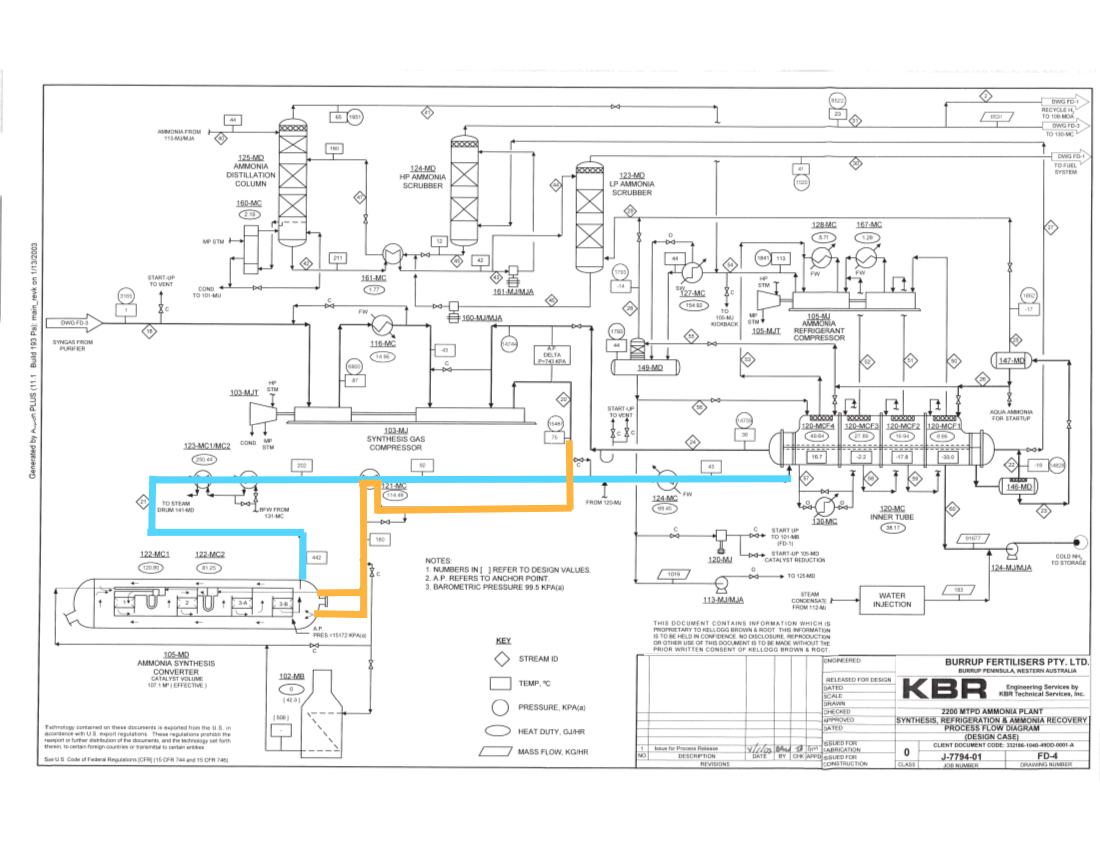
\includegraphics[scale=0.5]{task4/Plan1.png}
	\end{center}
	\caption{Circulation du flux}
	\label{cir1}
\end{figure}

\begin{figure}[h]
	\begin{center}
	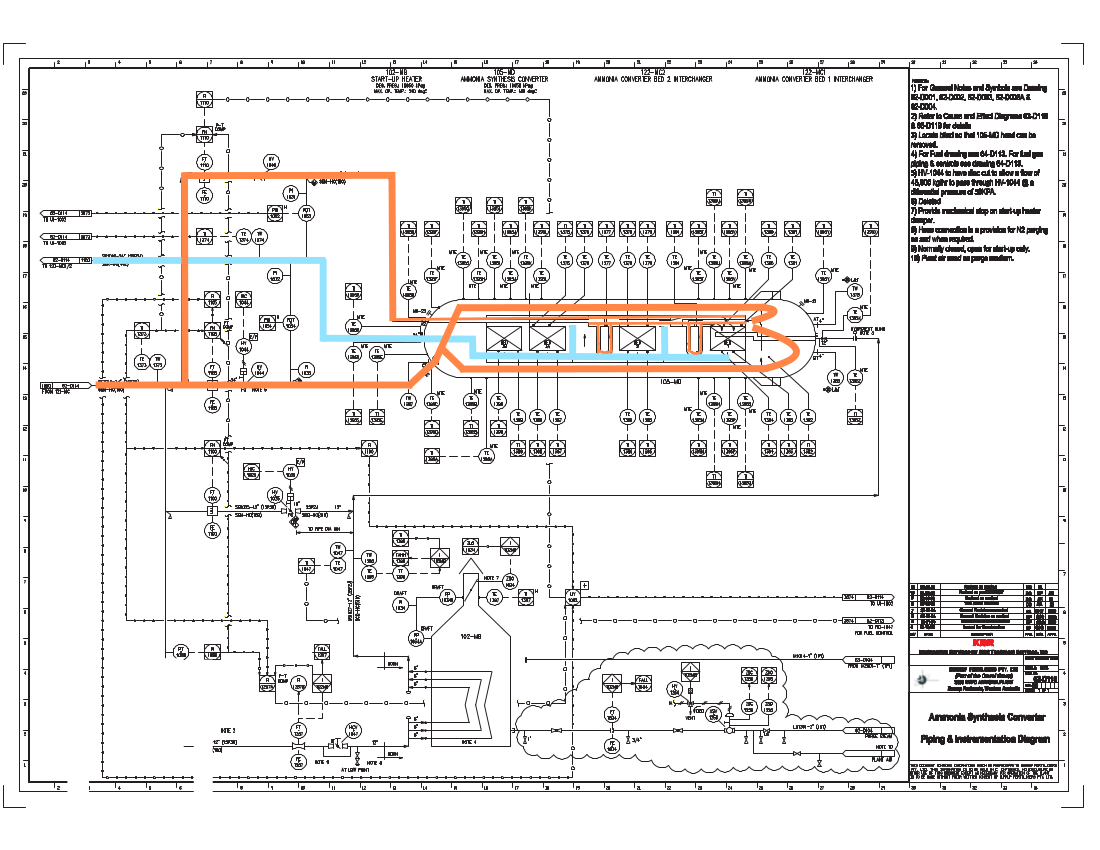
\includegraphics[scale=0.5]{task4/Plan2.png}
	\end{center}

	\caption{Circulation du flux}
	\label{cir2}
\end{figure}

\begin{figure}[h]
	\begin{center}
	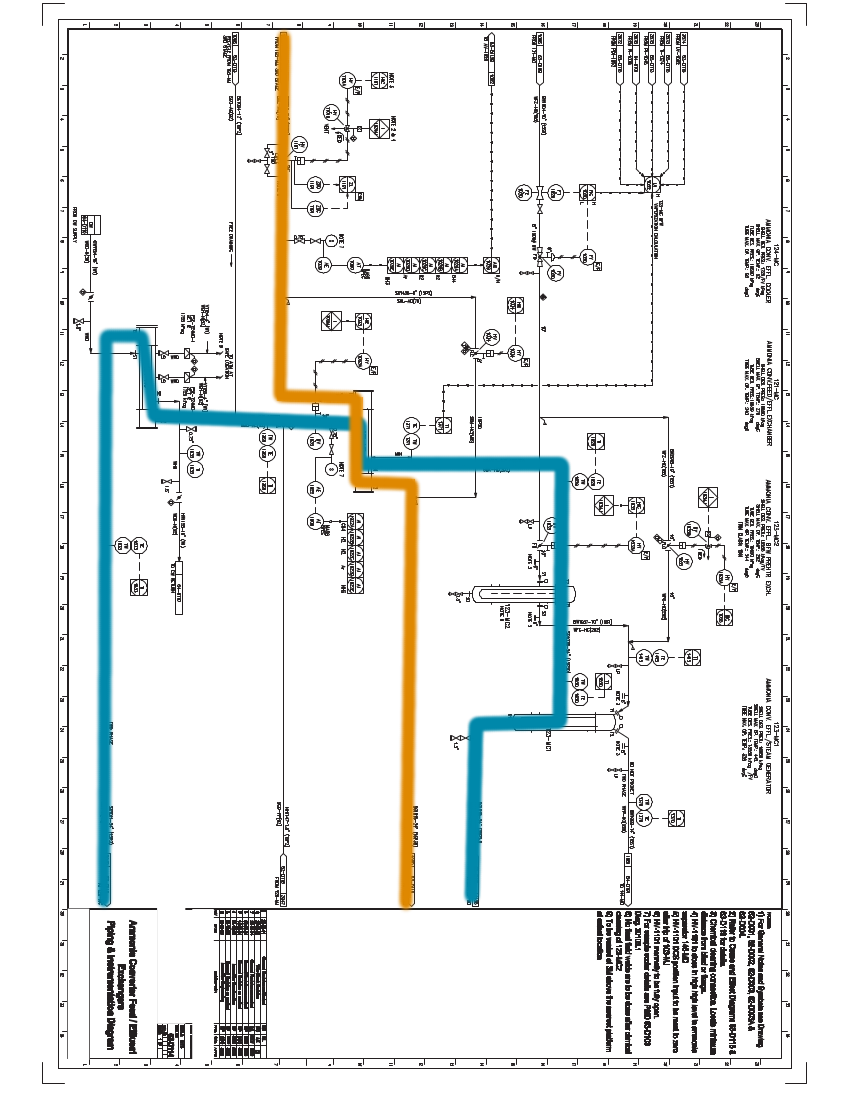
\includegraphics[scale=0.5]{task4/Plan2-2.png}
	\end{center}
	\caption{Circulation du flux}
	\label{cir3}
\end{figure}

\begin{figure}[h]
	\begin{center}
	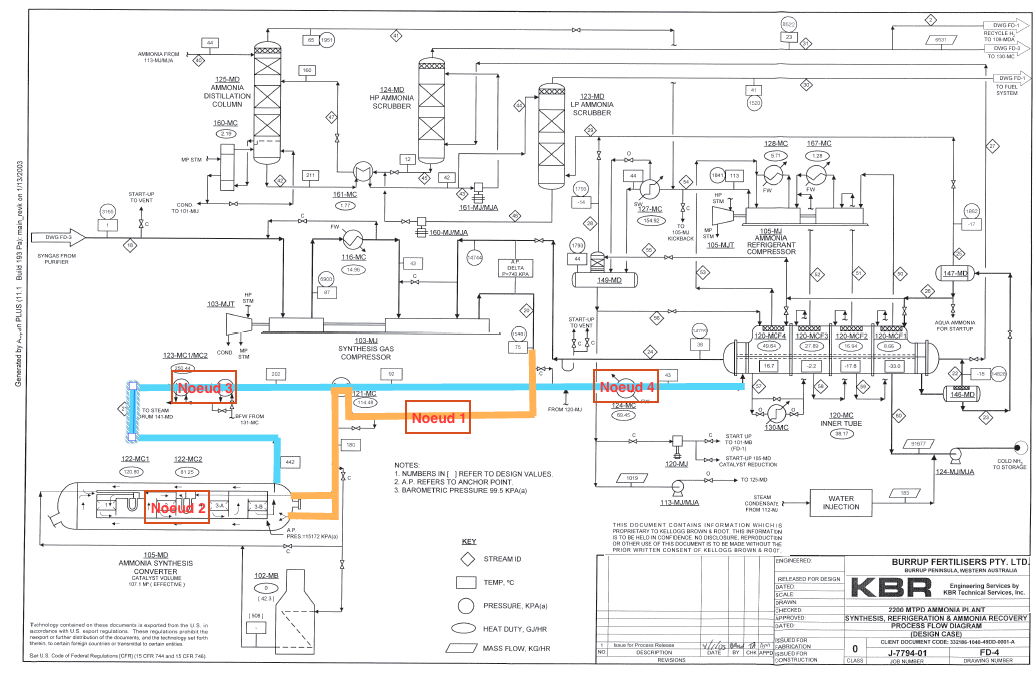
\includegraphics[scale=0.4]{task4/Position_des_differents_noeuds.png} 
	\end{center}
	\caption{Position des  Noeuds}
	\label{cir4}	
\end{figure}

\end{document}

\end{document}